\documentclass[14pt]{beamer}
\usepackage[T2A]{fontenc}
\usepackage[utf8]{inputenc}
\usepackage[english,russian]{babel}
\usepackage{amssymb,amsfonts,amsmath,mathtext}
\usepackage{cite,enumerate,float,indentfirst}


\graphicspath{{images/}}

\usecolortheme{seagull}

\setbeamercolor{footline}{fg=gray}
\setbeamertemplate{footline}{
  \leavevmode%
  \hbox{%
  \begin{beamercolorbox}[wd=1\paperwidth,ht=2.25ex,dp=1ex,right]{}%
  Стр. \insertframenumber{} из \inserttotalframenumber \hspace*{2ex}
  \end{beamercolorbox}}%
  \vskip0pt%
}

\newcommand{\itemi}{\item[\checkmark]}

\author{\small{%
Тема нашей презентации\\%
\vspace{50pt}
\emph{Выступающиe:}~П. С. Анашкевич, Р. И. Будный\\%
\emph{Руководитель:}~проф.,~к.ф.-м.н.~В.В.Цегельник}
\vspace{30pt}
}
\date{\small{Минск, 2013}}

\begin{document}

\maketitle



\begin{frame}
\frametitle{Постановка задачи}



\end{frame}



\begin{frame}

\frametitle{Определение}

Асинхронный двигатель --- электрическая машина переменного тока, частота вращения ротора которой не равна частоте вращения магнитного поля, создаваемого током обмотки статора.

%%Про беличью клетку

\end{frame}


\begin{frame}
\frametitle{Устройство}

\begin{figure}[H]
  \center
  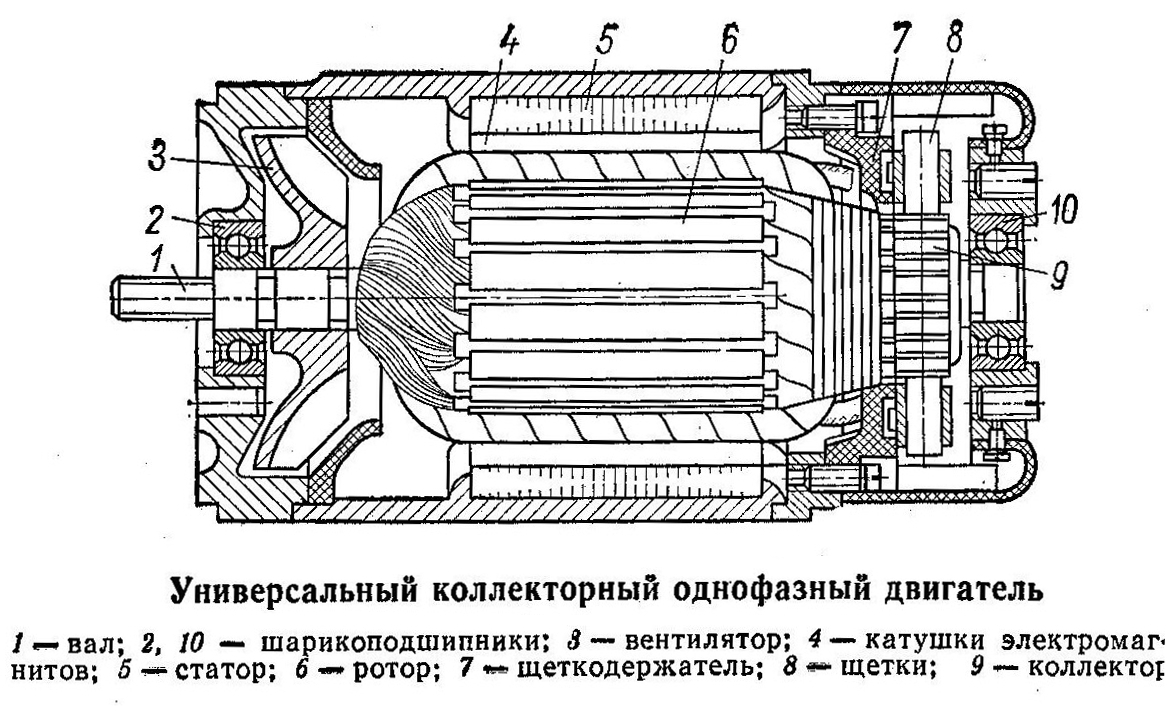
\includegraphics[width=0.8\linewidth]{konstrukciya-1}
\end{figure}

\end{frame}


\begin{frame}
\frametitle{Режимы работы}

\begin{figure}[H]
  \center
  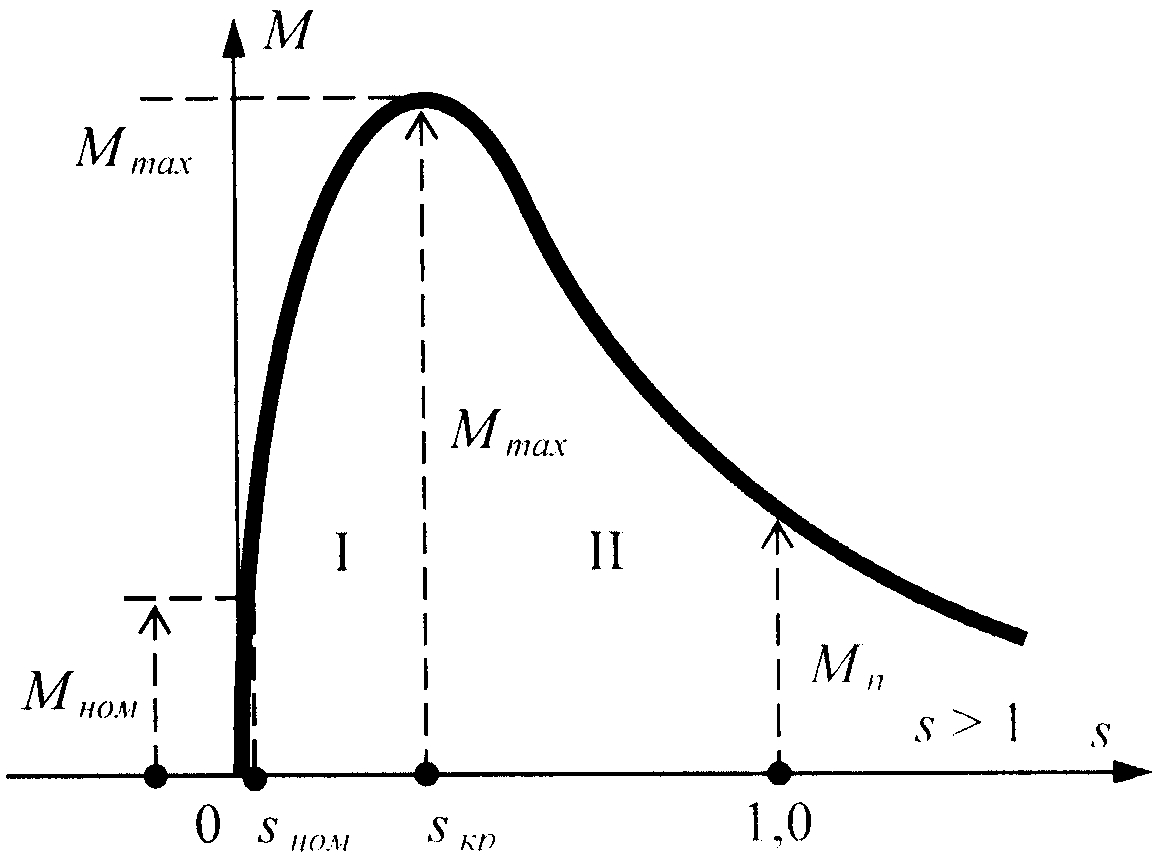
\includegraphics[width=0.6\linewidth]{zavisimost-1}
\end{figure}

\vspace{10pt}

\small{s -- скольжение: $ s = 1 - \dfrac{n}{n_c} $}	

\small{M -- крутящий момент}
	

\end{frame}




\begin{frame}
\frametitle{Поль Пенлеве}


\begin{figure}[H]
  \center
  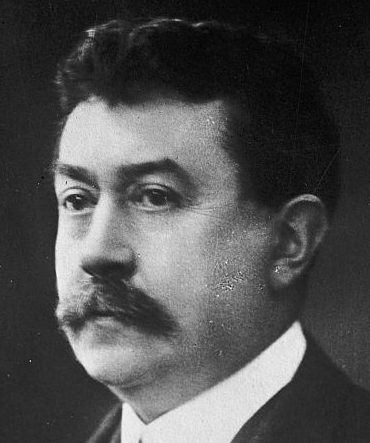
\includegraphics[width=0.4\linewidth]{penleve}
\end{figure}

\small{Французский математик и политик. Один из создателей аналитической теории дифференциальных уравнений.
}
\end{frame}


\begin{frame}

\frametitle{$\alpha $-метод Пенлеве}

Основан на методе малого параметра Пуанкаре. 

Используется для анализа дифференциальных уравнений. 

\end{frame}


\begin{frame}
\frametitle{Модель}

\begin{figure}[H] 
  \begin{center}

  \begin{minipage}[h]{0.4\linewidth}

  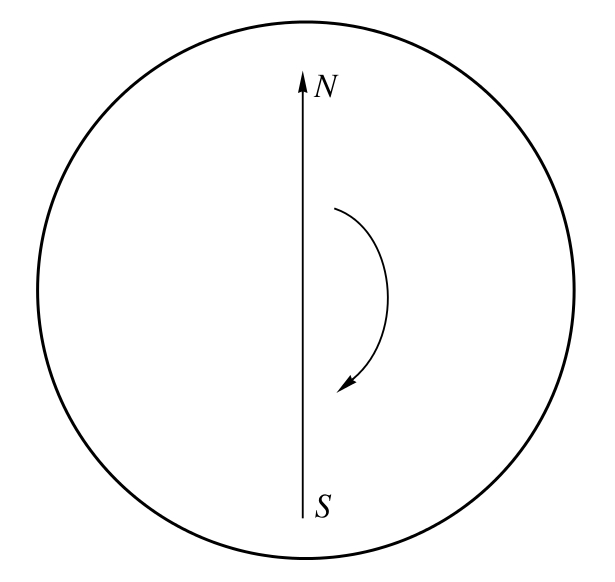
\includegraphics[width=1\linewidth]{magnitnoe_pole}

  \center{\small{Вращающееся \\ магнитное поле}}
  
  \end{minipage}
  \hfill   
  \begin{minipage}[h]{0.4\linewidth}
    
  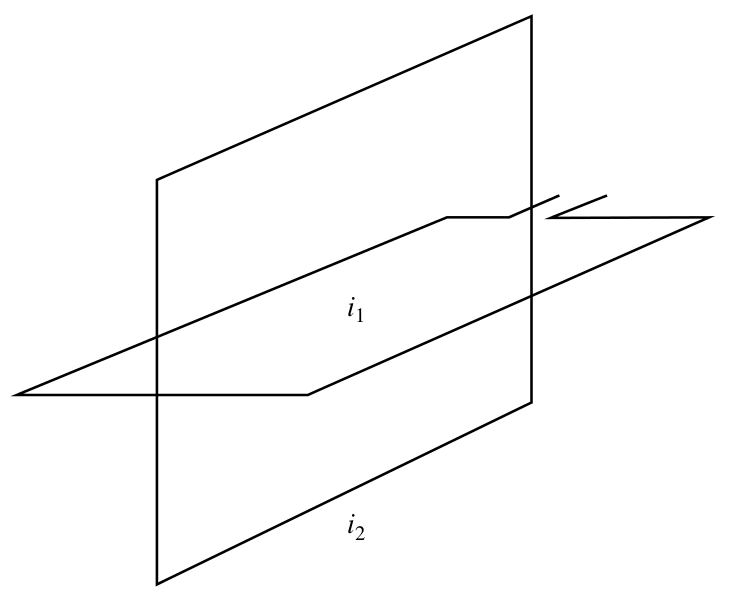
\includegraphics[width=1\linewidth]{obmotki}
  
  \center{\small{Схема обмоток}}
  \end{minipage}    
    
  \end{center}
\end{figure}


\end{frame}


\begin{frame}

\frametitle{Физическое описание}
$$
        \left\{
                \begin{aligned}
                        L \dfrac{di_1(t)}{dt} + Ri_1(t) = e + SB(\sin\theta(t)) \dot \theta (t), \\
                        L \dfrac{di_2(t)}{dt} + Ri_2(t) = e + SB(\cos\theta(t)) \dot \theta (t),
\\
  						I \ddot \theta = -\beta SB(i_1(t)\sin\theta + i_2(t)\cos\theta) - M.
                \end{aligned}
        \right.
$$
\end{frame}


\begin{frame}

\frametitle{Исходная система}
$$
        \left\{
                \begin{aligned}
                        \dot s &= ay + \gamma \\
                        \dot y &= -cy -s -xs \\
                        \dot x &= cx + ys
                \end{aligned}
        \right. 
$$

\vspace{10pt}

\small{

где $ s = \dot \theta_1 = \dot{(-\theta)}, a = \dfrac{\beta(SB)^2}{IL}, c = \dfrac{R}{L}, $

\hspace{15pt} $ x = \dfrac{L}{SB} (i_1\cos\theta_1 + i_2\sin\theta_1),$

\vspace{5pt}

\hspace{15pt} $ y = \dfrac{L}{SB} (-i_1\sin\theta_1 + i_2\cos\theta_1).$
}

\end{frame}



\begin{frame}

\frametitle{Метод Пенлеве: шаг 1}

\small{Пусть $ s = \dfrac{s_0}{\tau^k}, y = \dfrac{y_0}{\tau^l} , x = \dfrac{x_0}{\tau^m} $:}
\vspace{10pt}
$$      
         \left\{
                \begin{aligned}
                        -\dfrac{ks_0}{\tau^{k+1}} &= a \dfrac{y_0}{\tau^l} + \gamma \\
                        -\dfrac{ly_0}{\tau^{l+1}} &= -c \dfrac{y_0}{\tau^l} - \dfrac{s_0}{\tau^k} - \dfrac{x_0}{\tau^m} \dfrac{s_0}{\tau^k} \\
                        -\dfrac{mx_0}{\tau^{m+1}} &= -c \dfrac{x_0}{\tau^m} + \dfrac{y_0}{\tau^l} \dfrac{s_0}{\tau^k}
                \end{aligned}
        \right.
$$

\end{frame}



\begin{frame}

\frametitle{Метод Пенлеве: шаг 1}

\small{
$$
        \left\{
                \begin{aligned}
                        -\dfrac{s_0}{\tau^2} &= a \dfrac{y_0}{\tau^2} + \gamma \\
                        -\dfrac{2y_0}{\tau^3} &= -c \dfrac{y_0}{\tau^2} - \dfrac{s_0}{\tau} - \dfrac{x_0 s_0}{\tau^3} \\
                        -\dfrac{2x_0}{\tau^{3}} &= -c \dfrac{x_0}{\tau^2} + \dfrac{y_0 s_0}{\tau^3}
                \end{aligned}
        \right.
$$
}

откуда получим, что:

\vspace{10pt}

\begin{minipage}[h!]{0.4\linewidth}
$$
\label{eq:step2_a}
\left\{
\begin{aligned}
  x_0 &= - \dfrac{2}{a} \\
  y_0 &= -\dfrac{2i}{a} \\
  s_0 &= 2i \\
\end{aligned}
\right.
$$
\end{minipage}
\hfill
либо
\hfill
\begin{minipage}[h!]{0.4\linewidth}
$$
\label{eq:step2_b}
\left\{
\begin{aligned}
  x_0 &= - \dfrac{2}{a} \\
  y_0 &= \dfrac{2i}{a} \\
  s_0 &= - 2i
\end{aligned}
\right.
$$
\end{minipage}


\end{frame}

\begin{frame}

\frametitle{Метод Пенлеве: шаг 2}

\small{Сделаем подстановку в виде
 
\vspace{10pt} $ 
s = \dfrac{s_0}{\tau} + \alpha \tau^{r-1},
y = \dfrac{y_0}{\tau^2} + \beta \tau^{r-2},                         x = \dfrac{x_0}{\tau^2} + \theta \tau^{r-2} $:

$$
        \left\{
                \begin{aligned}
                        -\dfrac{s_0}{\tau^{2}} + \alpha (r-1) \tau^{r-2} &= a \left( \dfrac{y_0}{\tau^2} + \beta \tau^{r-2} \right) + \gamma \\
                        -\dfrac{2y_0}{\tau^{3}} + \beta (r-2) \tau^{r-3} &= -c \left( \dfrac{y_0}{\tau^2} + \beta \tau^{r-2} \right) - \left( \dfrac{s_0}{\tau} + \alpha \tau^{r-1} \right) - \\ &- \left( \dfrac{x_0}{\tau^2} + \theta \tau^{r-2} \right) \left( \dfrac{s_0}{\tau} + \alpha \tau^{r-1} \right) \\
                        -\dfrac{2x_0}{\tau^{3}} + \theta (r-2) \tau^{r-3} &= -c \left( \dfrac{x_0}{\tau^2} + \theta \tau^{r-2} \right) + \\ &+ \left( \dfrac{y_0}{\tau^2} + \beta \tau^{r-2} \right) \left( \dfrac{s_0}{\tau} + \alpha \tau^{r-1} \right)
                \end{aligned}
        \right.
$$
}

\end{frame}



\begin{frame}

\frametitle{Метод Пенлеве: шаг 2}

Составим матрицу из коэффициентов при $ \alpha $, $ \beta $, $ \theta $:

$$
\left(
                \begin{array}{ccc}
                        r-1 & -a & 0 \\
                        x_0 & r-2 & s_0 \\
                        -y_0 & -s_0 & r-2 \\
                \end{array}
\right)
$$

Определитель приравняем к нулю, откуда получим:

\center{$ r_1 = - 1, r_2 = 2, r_3 = 4 $.}

\end{frame}



\begin{frame}

\frametitle{Метод Пенлеви: шаг 3}

$$
        \left\{
                \begin{aligned}
                        s &= \dfrac{s_{-1}}{\tau} + s_0 + s_1\tau + s_2\tau^2 + s_3\tau^3 + \ldots \\
                        y &= \dfrac{y_{-2}}{\tau^2} + \dfrac{y_{-1}}{\tau} + y_0 + y_1\tau + y_2\tau^2 + y_3\tau^3 + \ldots \\
                        x &= \dfrac{x_{-2}}{\tau^2} + \dfrac{x_{-1}}{\tau} + x_0 + x_1\tau + x_2\tau^2 + x_3\tau^3 + \ldots
                \end{aligned}
        \right.
$$
\end{frame}
%
%
%
%\begin{frame}
%
%\frametitle{Метод Пенлеви: шаг 3}
%
%Корни уравнения.
%
%\end{frame}
%
%
%
%\begin{frame}
%
%\frametitle{Метод Пенлеви: шаг 4}
%
%Описание подстановки.
%
%\end{frame}
%
%
%\begin{frame}
%
%\frametitle{Метод Пенлеви: шаг 4}
%
%Полученные коэффициенты.
%
%\end{frame}
%
%
%\begin{frame}
%
%\frametitle{Анализ решения}
%
%Анализ решения системы.
%
%\end{frame}
%
%\begin{frame}
%
%\frametitle{Выводы}
%
%Выводы
%
%\end{frame}
%

\begin{frame}
\begin{center}
Спасибо за внимание!
\end{center}
\end{frame}

\end{document} 
